\documentclass{beamer}
\usepackage{changepage}
\usepackage{multicol}

\usetheme[numbering=fullbar]{focus}

\definecolor{main}{RGB}{92, 138, 168}

\title{The Ultimate Keyboard}
\subtitle{A Genetic Algorithm}
\author{Aniruddh Mishra}
\institute{Institute for Computing in Research}
\date{\today}

\begin{document}
    \begin{frame}
        \maketitle
    \end{frame}

    \begin{frame}{Overview}
        \vspace{-5em}
        \begin{adjustwidth}{3em}{-1em}
            \setbeamertemplate{section in toc}[sections numbered]
            \begin{multicols}{2}
                \setlength{\parskip}{2em}
                \tableofcontents
            \end{multicols}
        \end{adjustwidth}
    \end{frame}
    
    \section{Introduction}

    \begin{frame}{Keyboards}
        \begin{figure}
            \centering
            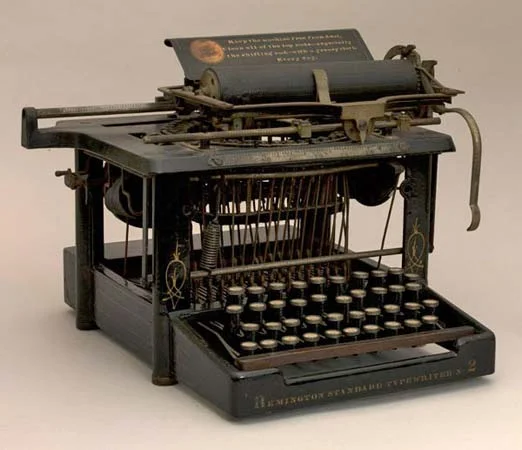
\includegraphics[width=15em, keepaspectratio]{images/typewriter.png}
            \caption{Typewriter \cite{typewriter}}
        \end{figure}
    \end{frame}

    \section{Genetic Algorithms}

    \begin{frame}{Stochastic Approximation}
        \begin{figure}
            \centering
            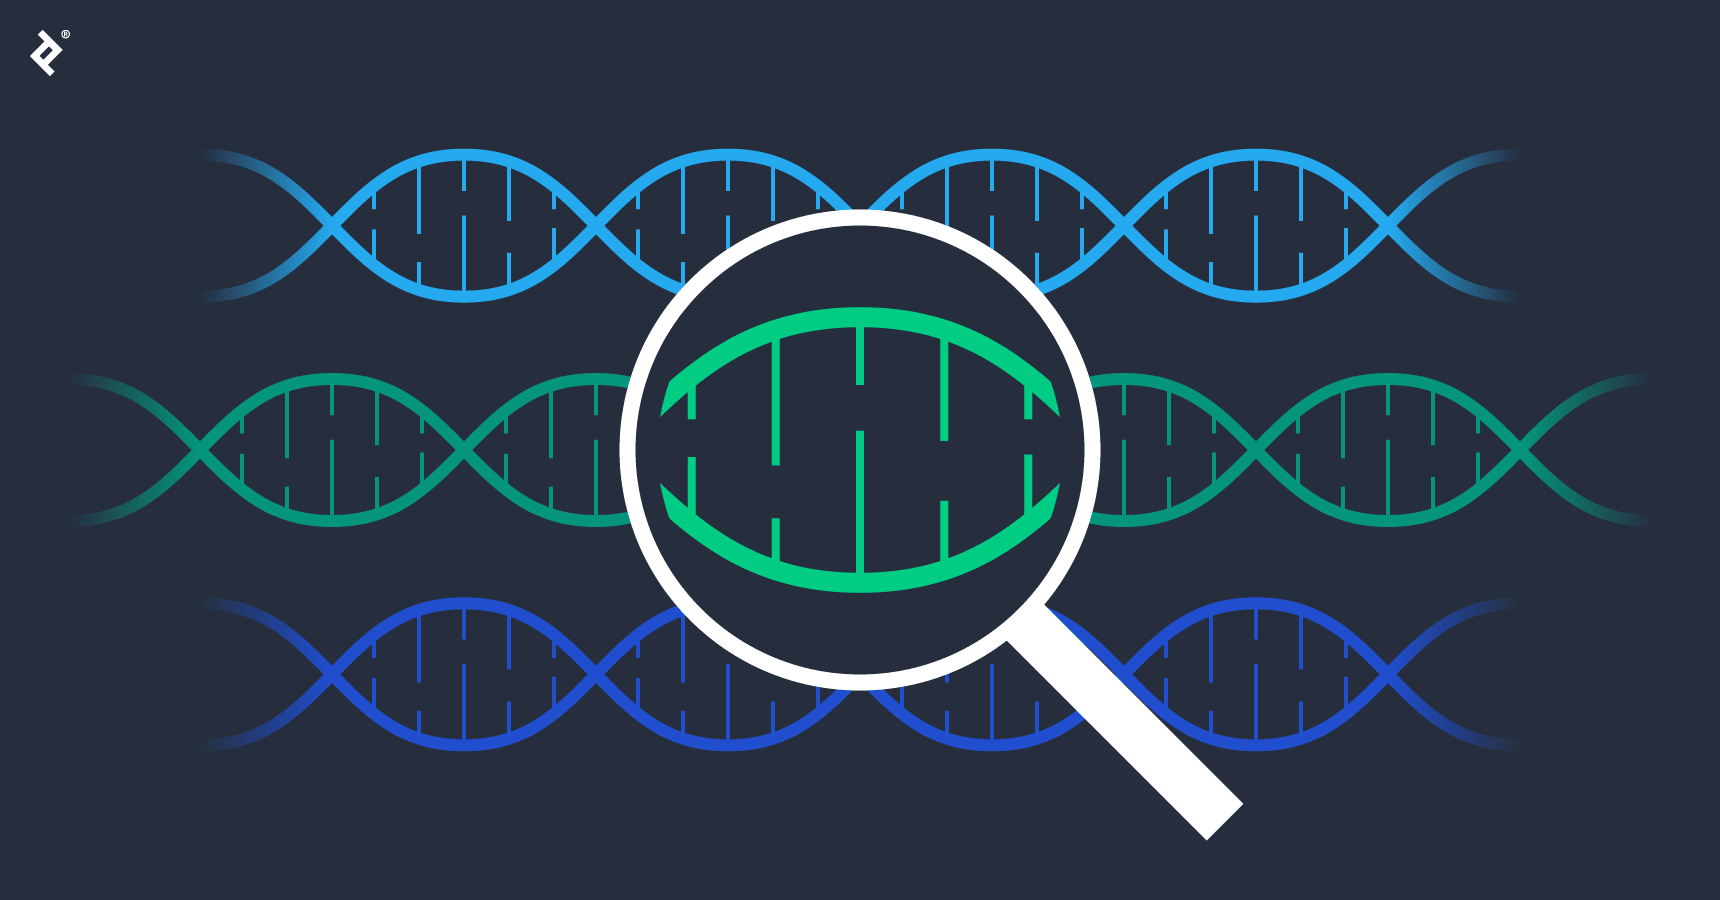
\includegraphics[width=20em, keepaspectratio]{images/genetic.png}
            \caption{Image of DNA \cite{genetic}}
        \end{figure}
    \end{frame}

    \section{Keyboard Fitness}
    % Typing Styles
    \begin{frame}{Typing Styles}
        \begin{figure}
            \centering
            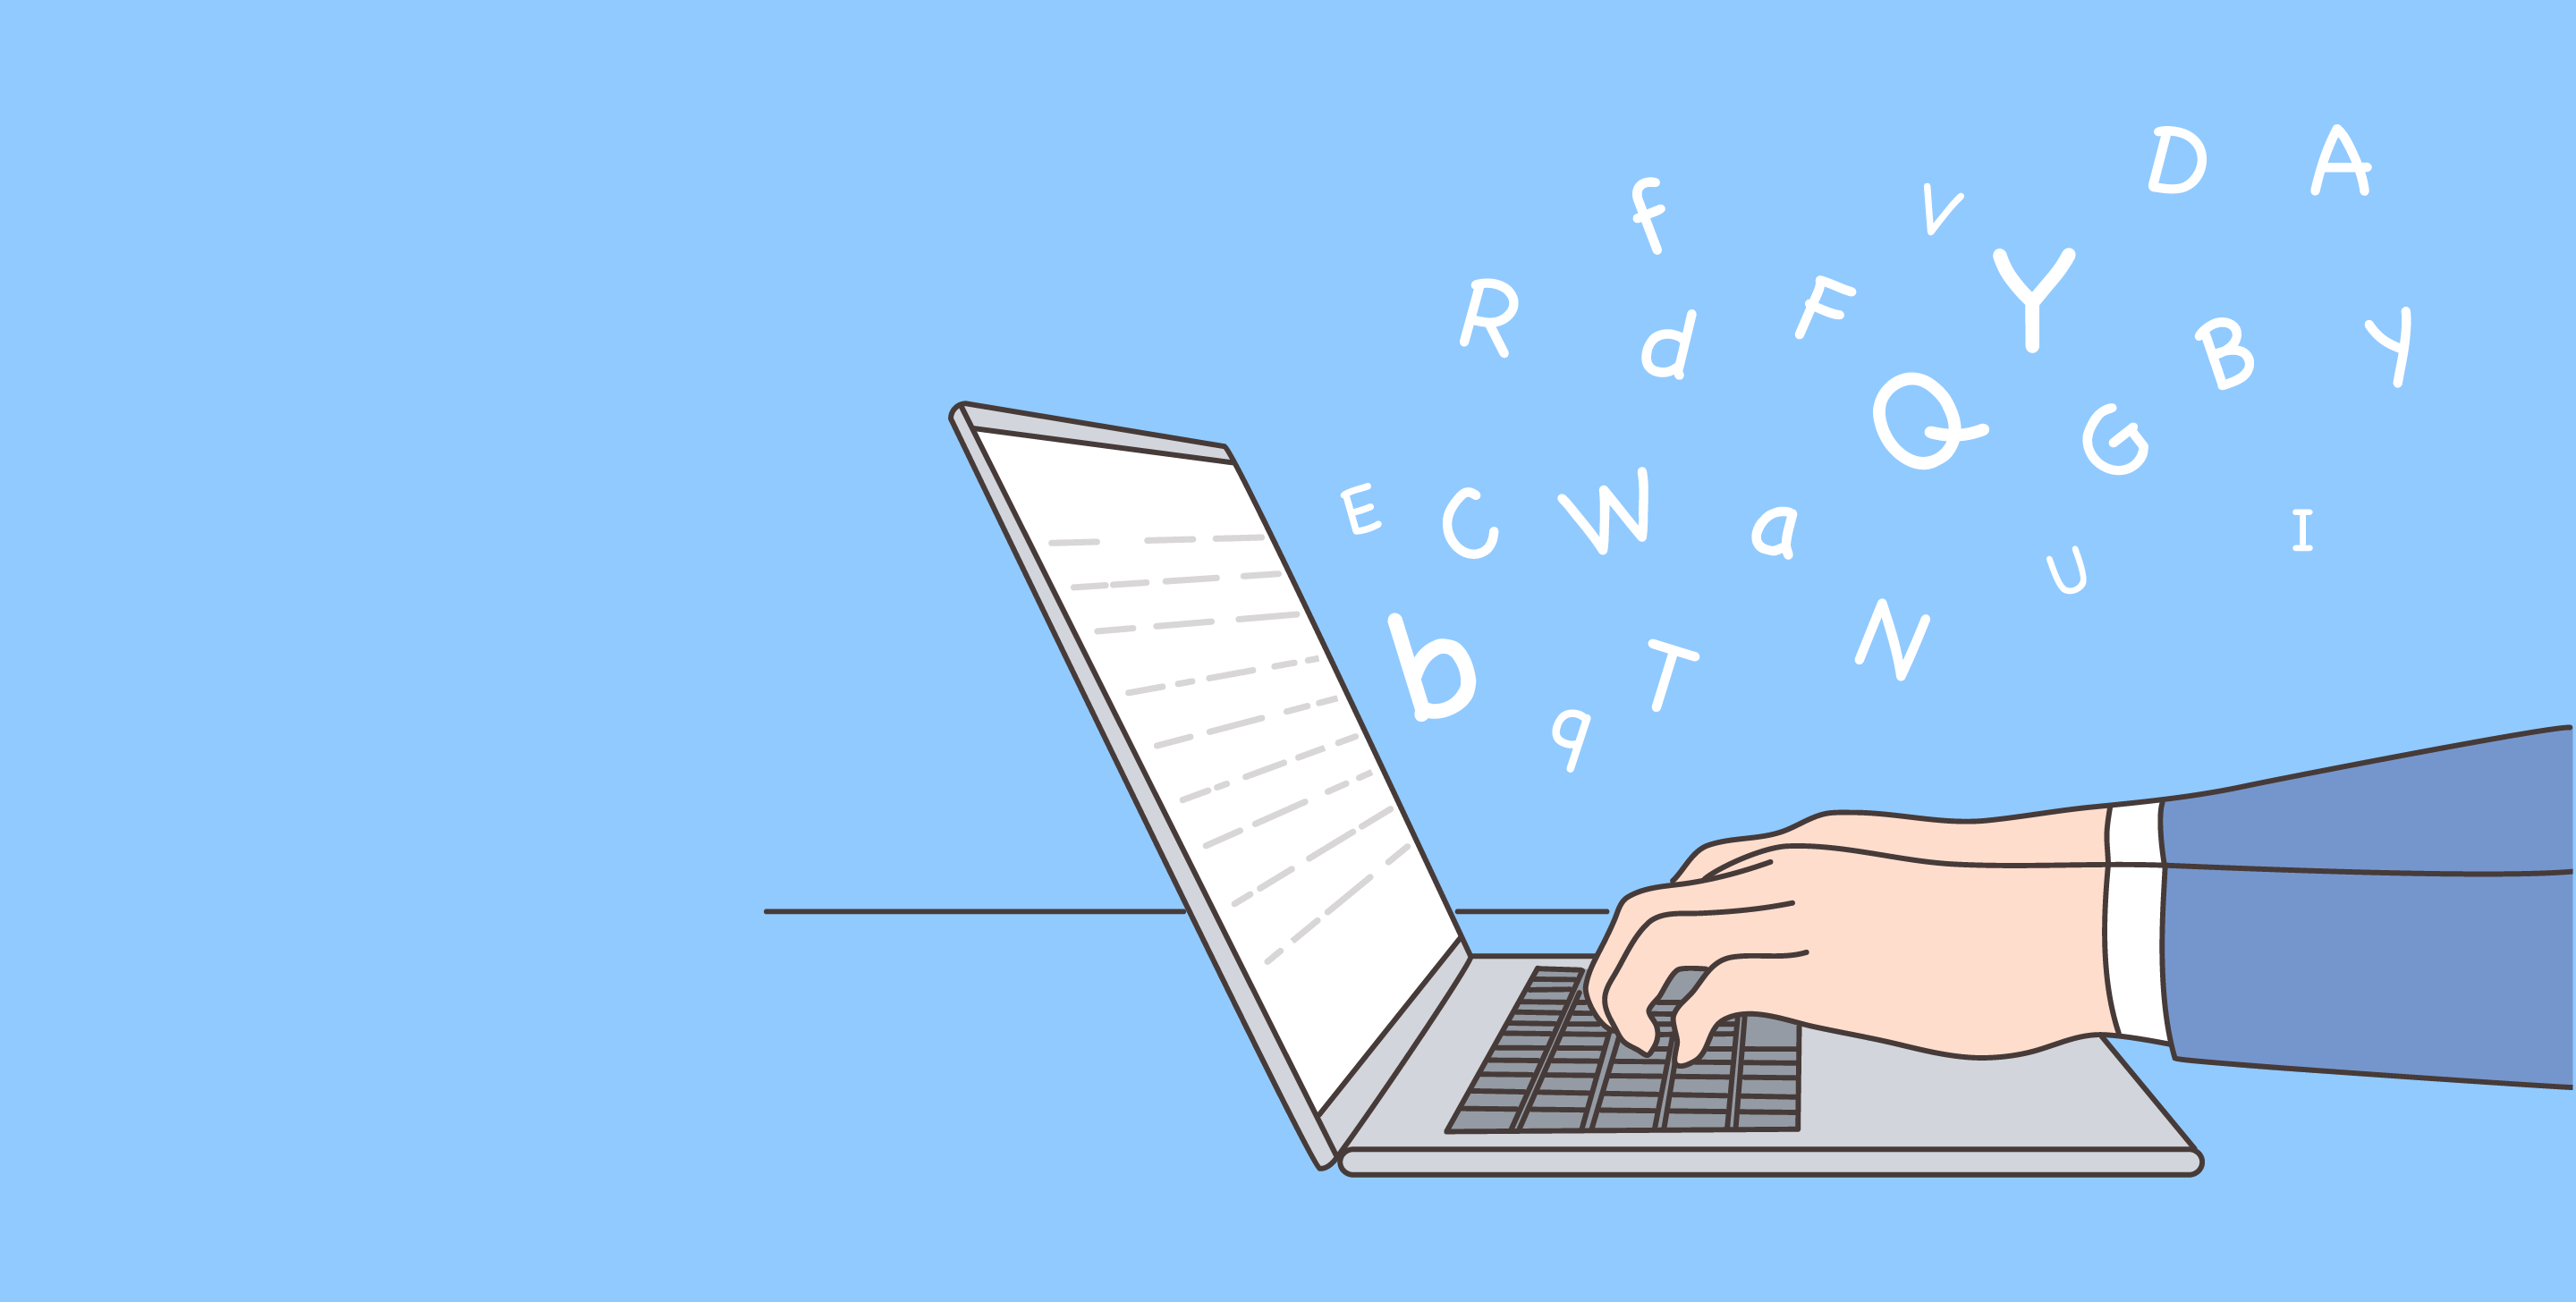
\includegraphics[width=20em, keepaspectratio]{images/typing.png}
            \caption{Illustration of typing \cite{typing}}
        \end{figure}
    \end{frame}

    \begin{frame}{Bee Movie}
        \begin{figure}
            \centering
            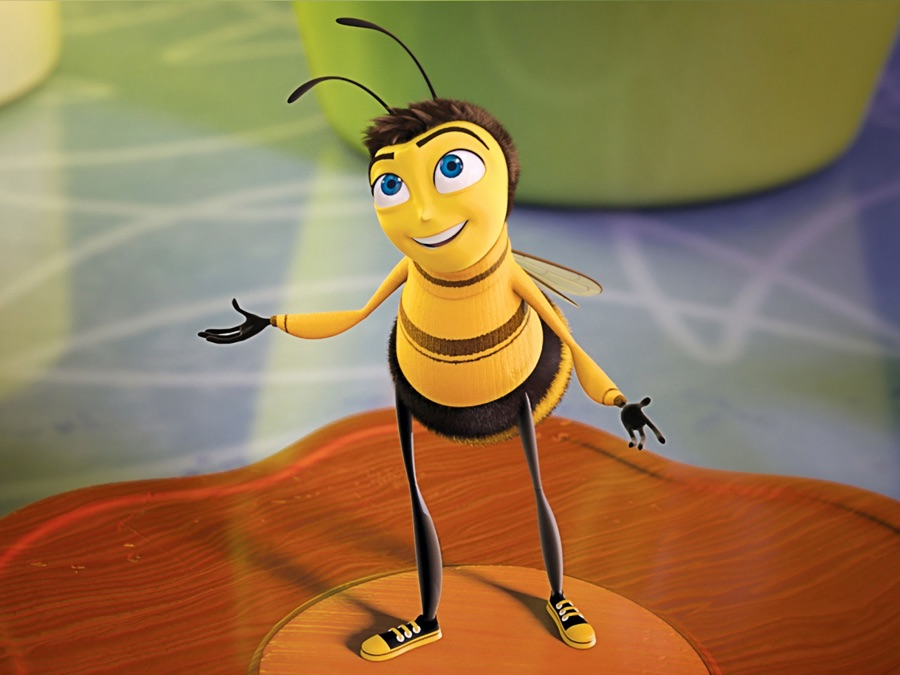
\includegraphics[width=15em, keepaspectratio]{images/beeMovie.jpg}
            \caption{Scene from The Bee Movie \cite{bee-movie}}
        \end{figure}
    \end{frame}

    \section{Experiments}

    \begin{frame}{Hi}
        \begin{figure}
            \centering
            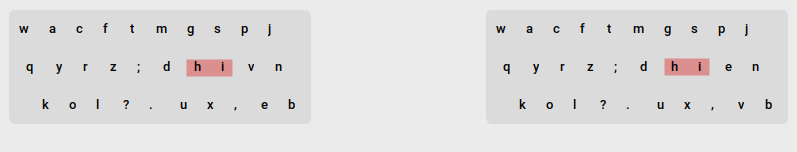
\includegraphics[width=25em, keepaspectratio]{images/hiRfp.png}
            \caption{Keyboard output for sample word "hi"}
        \end{figure}
    \end{frame}

    \begin{frame}{Hello World}
        \begin{figure}
            \centering
            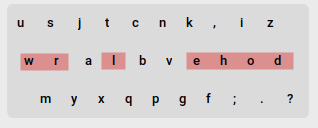
\includegraphics[width=20em, keepaspectratio]{images/helloWorld.png}
            \caption{Keyboard output for sample "hello world"}
        \end{figure}
    \end{frame}

    \begin{frame}{Bee Movie Keyboard}
        \begin{figure}
            \centering
            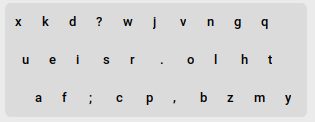
\includegraphics[width=20em, keepaspectratio]{images/beeMovieKeyboard.png}
            \caption{Keyboard output for sample "hello world"}
        \end{figure}
    \end{frame}

    \begin{frame}{Ultimate Keyboard}
        \begin{figure}
            \centering
            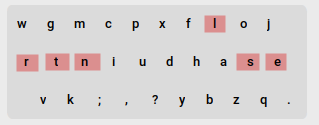
\includegraphics[width=20em, keepaspectratio]{images/ultimateKeyboard.png}
            \caption{Keyboard output for sample "hello world"}
        \end{figure}
    \end{frame}
    
    \section{Conclusion}

    \begin{frame}{What's Next?}
        \begin{figure}
            \centering
            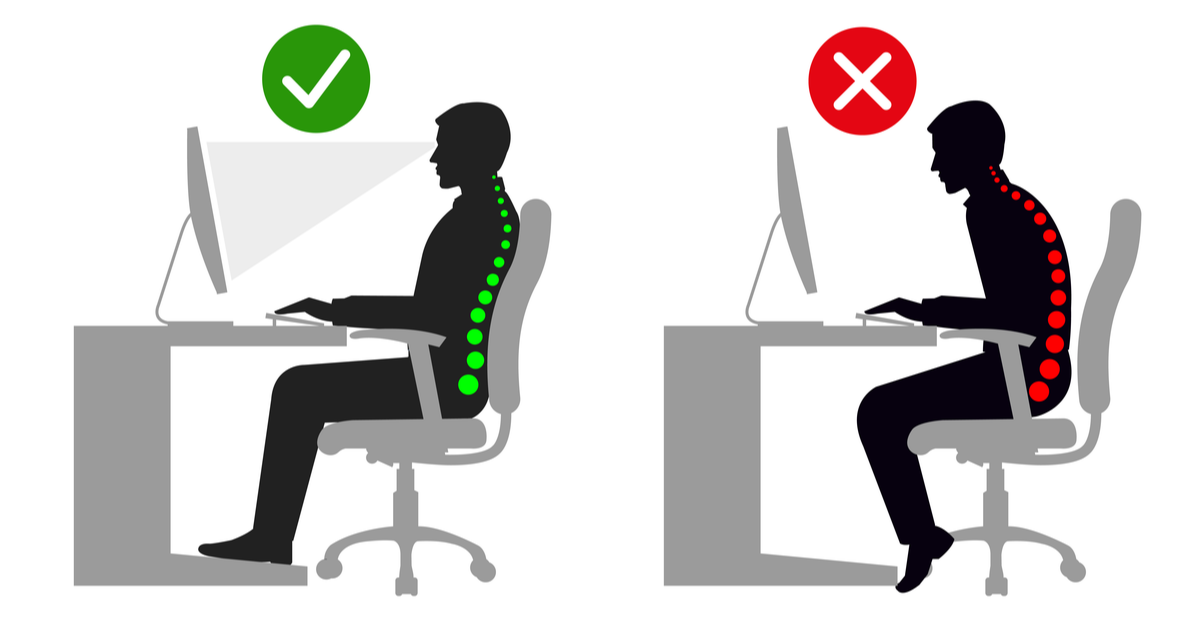
\includegraphics[width=20em, keepaspectratio]{images/ergonomic.png}
            \caption{Ergonomics for keyboards \cite{ergonomics}}
        \end{figure}
    \end{frame}

    \section{Questions}
    
    \begin{frame}[allowframebreaks]{References}
        \bibliography{bibliography}
        \bibliographystyle{abbrv}
    \end{frame}
    
\end{document}
